\documentclass{article}
\usepackage{ctex}%引入中文宏包
\usepackage{hyperref}%超链接
\usepackage{color}%字体颜色
\usepackage{geometry}
\usepackage{indentfirst}%首行缩进
\usepackage{amssymb}%数学
\usepackage{amsmath}
\usepackage{graphicx}%插入图片
\usepackage{multirow}%合并行列
\usepackage{fancyhdr}%页眉页脚
\usepackage{listings}%插入代码
\usepackage{float}%浮动插入内容,不会使后面的内容跑到前面去(在插入的begin后面加上H)
\usepackage{bm}
\usepackage{xeCJK}

\setlength{\parindent}{\ccwd}
\geometry{left=2.54cm, right=2.54cm, top=3.18cm, bottom=3.18cm}
\linespread{1.5}
\pagenumbering{roman}
\setCJKfamilyfont{song}{SimSun} 

\title{\heiti 数值分析中期报告}
\author{陈高明 \quad 梁浩贤 \quad 汪泓宇}
\date{\today}

\begin{document}
\newtheorem{theorem}{定理}[section]
\newtheorem{definition}[theorem]{定义}
\newtheorem{lemma}[theorem]{引理}
\newtheorem{corollary}[theorem]{推论}
\newtheorem{example}[theorem]{例}
\newtheorem{proposition}[theorem]{命题}
    \maketitle

    \begin{abstract}
        最佳平方逼近是函数逼近论中的重要课题,本质上它研究函数在$L^2$范数意义下的收敛序列。
        在多项式最佳平方逼近中,以正交多项式作为逼近函数空间的基有许多好处,
        如在增加多项式的次数后,最佳逼近多项式只需增加一项新的正交多项式的常数倍,
        而对于之前的正交多项式的组合系数并不改变。最大误差研究函数在$L^\infty$范数意义下的收敛性。
        
        然而不幸的是,函数在$L^2$意义下的收敛性无法推出$L^\infty$收敛,这往往需要单独的证明。
        我们研究在区间$[-1,1]$上,用勒让德多项式函逼近数$f(x)=e^x$。在编程中使用python的sympy包,
        计算过程都为解析的。本文利用递推关系计算了38次勒让德多项式的解析解,并求解
        $f$的各次最佳平方逼近函数的解析解。随后计算了这些最佳平方逼近多项式的最大误差,
        并利用数值试验猜测他们和$n$的函数关系,并进行理论证明。最终,我们的数值试验和理论证明表明,
        $f(x)=e^x$在勒让德多项式的平方逼近下,最大误差收敛速度为$O((\frac{e}{2n})^n).$ \\
        \noindent{\textbf{关键词:}}
    \end{abstract}
    
    \section{计算最佳平方逼近的m次多项式}
    本次实验,我们需要利用勒让德正交多项式$\varphi_n(x)=\frac{1}{n!2^n}\frac{d^n}{dx^n}(x^2-1)^n$,构造最佳逼近函数。
    \par
    我们首先需要利用所学知识,根据勒让德多项式的递推关系$(k+1)\varphi_{k+1}(x)=(2k+1)x\varphi_k(x)-k\varphi_{k-1}(x)$,构造出$k+1$阶勒让德多项式的表达式。
    这样做的目的是为了避免求微分的运算过于繁琐,增加运算量,若使用递推公式,则只涉及到$O(n)$次的乘法运算。
    \par
    为了避免分数转化为小数的误差,在求勒让德多项式的过程中,我们使用了准确的分数表示勒让德多项式的各项系数(以下称其为解析的)。
    接着,我们计算$k$阶勒让德多项式的模长$(\varphi_k(x),\varphi_k(x))$,$k$阶勒让德多项式与目标函数的内积$(\varphi_k(x),f(x))$。两者的计算均使用软件上相应的程序包,
    该程序包可以对初等函数简单组合的积分求解析的原函数。得到以上结果后,利用课件上的公式$P_n(x)=\sum_{k=0}^{n}\frac{(f,\varphi_k)}{(\varphi_k,\varphi_k)}\varphi_k(x)$,
    得到$P_n(x)$的解析表达式(此时未将目标函数与多项式内积中的$e$的次方项化为小数形式)。最后得到误差表达式$f(x)-P_n(x)$,
    并将$[-1,1]$代入求得误差的绝对值,根据绝对值画出误差曲线。(步长0.01)


    \section{误差收敛性估计}
    首先我们观察勒让德多项式逼近结果的误差与多项式空间的维数n的关系:
    \begin{figure}[H]
        \centering
        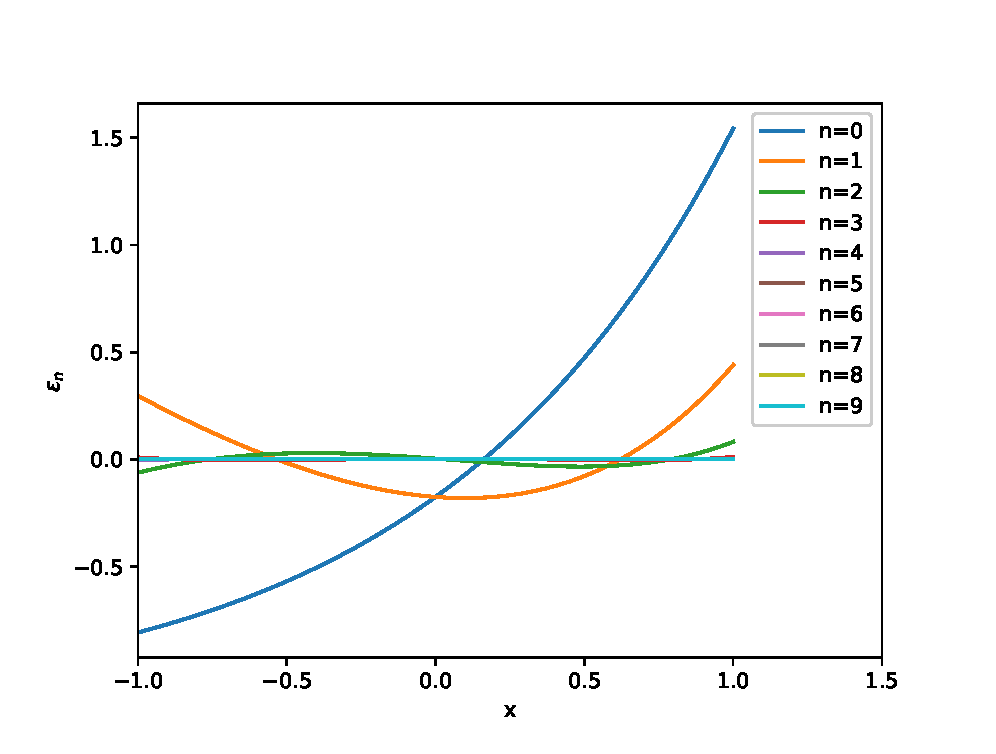
\includegraphics{epsilon.eps}
        \caption{p1}
    \end{figure}
    从图中可看出,误差以较快的速度衰减到0.这里我们采用最小二乘法(线性回归)来拟合误差:\\
    一般模型:
    $\varepsilon \sim \beta_0+\beta_1f_1(n)+\beta_2f_2(n)+\cdots+\beta_kf_k(n)$\\
    设$f_i(k),(k=1,2,\cdots,n)$为向量$x_i=(\xi_i^1,\xi_i^2,\cdots,\xi_i^n)^T$,
    $\varepsilon$的样本点为$Y=(y_1,y_2,\cdots,y_n)^T$,\\
    $X=(1_n,x_1,x_2,\cdots,x_k)$,
    $\beta=(\beta_0,\beta_1,\cdots,\beta_k)^T$,\\
    $\therefore \quad Y=X\beta+u$,$\beta=(X^TX)^{-1}X^TY$.其中
    $$
    X=\begin{bmatrix}
        1 & f_1(0) & f_2(0) & \cdots & f_k(0)\\
        1 & f_1(1) & f_2(1) & \cdots & f_k(1)\\
        1 & f_1(2) & f_2(2) & \cdots & f_k(2)\\
        \vdots & \vdots & \vdots & \ddots & \vdots \\
        1 & f_1(n) & f_2(n) & \cdots & f_k(n)
    \end{bmatrix}
    $$
    一般情况下$k<n$,当$\{f_1,f_2,\cdots,f_n\}$不相关时,$X$为列满秩,故$X^TX$为$k+1$阶可逆矩阵.
    因此系数估计$\beta$存在.

    \subsection{以指数速度收敛}
    即$error\sim e^{-n}$,仅对error求对数得$ln(error)\sim n$,
    
    \begin{figure}[H]
    	\centering
    	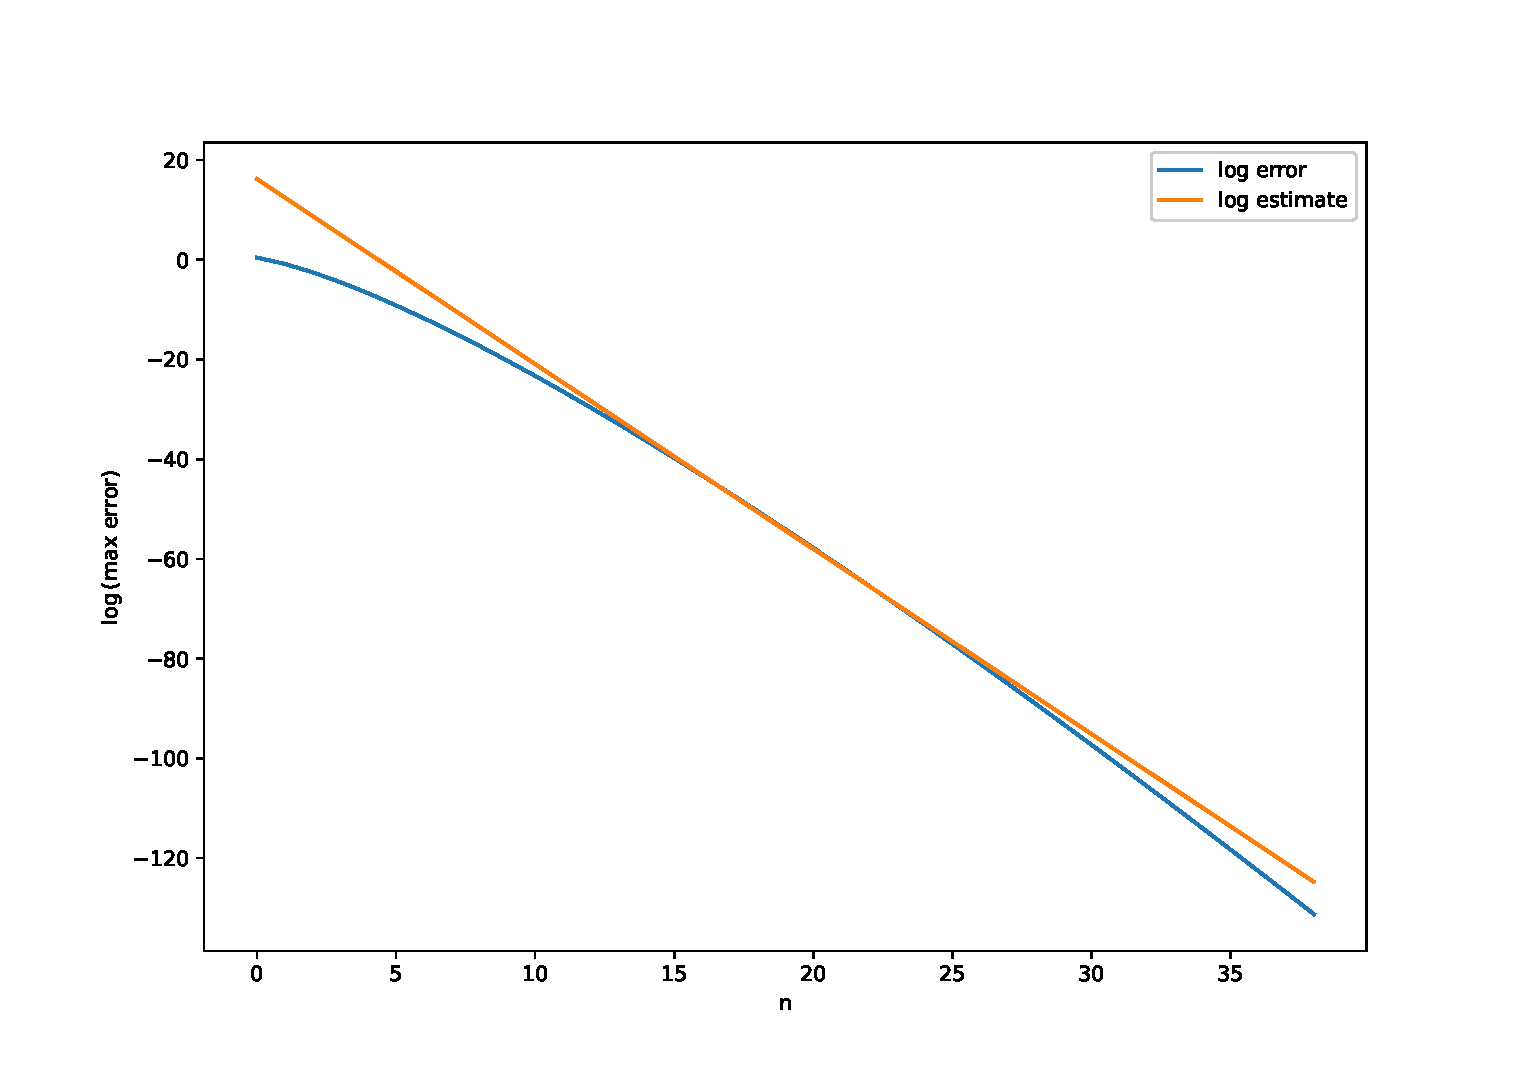
\includegraphics[width = 16cm]{linear regression of logerror to n.eps}
    	\caption{}
    \end{figure}

    \subsection{以指数的多项式速度衰减}
    即$error\sim e^{n^{k}}$对error求两次对数得$ln(ln(error))\sim n$,

    \subsection{最终模型}
    易见,上述的几种模型都不能很好地拟合数据,当多项式空间维数足够高的时候会出现较大偏差,
    并且从图像的趋势可以看出实际收敛速度更快,因此,我们小组尝试采用先理论推导后数值验证
    的方法进行探索:
    \par
    首先设函数$f(x)$在$[-1,1]$上连续,因此$\exists M>0, s.t. |f(x)|\leqslant M $. 记
    勒让德多项式空间为$span\{\varphi_1(x),\varphi_2(x),\cdots,\varphi_n(x)\}$, $f(x)$
    的n阶勒让德多项式逼近函数为$P_n(x)=\sum_{k=1}^{n} a_k\varphi_k(x) $, 其中
    $$a_k=\frac{\int_{-1}^{1} f(x)\varphi_k(x)\,dx}{\int_{-1}^{1} \varphi_k^2(x)\,dx}
    =\frac{2k+1}{2}\int_{-1}^{1} f(x)\varphi_k(x)\,dx
    $$
    记$\varepsilon_n=\mathop{max}\limits_{-1\leqslant x\leqslant 1}|f(x)-P_n(x)|$.\\
    \par
    我们小组通过数值实验得出,在$f(x)=e^x$时,$\varepsilon_n$在边界上取得,即$x=\pm 1$时
    误差取得最大值,而$P_n(1)=\sum_{k=0}^{n} a_k,\quad P_n(-1)=\sum_{k=0}^{n} (-1)^n a_k$
    因此$\varepsilon_n=|f(1)-P_n(1)|=|e-\sum_{k=0}^{n} a_k$| 或 
    $ \varepsilon_n=|f(-1)-P_n(-1)|=|e^{-1}-\sum_{k=0}^{n} (-1)^n a_k|$,故
    $|\varepsilon_n|\leqslant \sum_{k=0}^{n} |a_k|$,因此$\varepsilon_n$的收敛性可以被
    $\sum_{k=0}^{n} |a_k|$所控制.\\
    下面我们给出$a_n$的估计:\\
    \begin{lemma}
        记$g_n=(x^2-1)^n$,则对$\forall 1\leqslant k \leqslant n-1$,$g_n^{(k)}(1)=
        g_n^{(k)}(-1)=0$.
    \end{lemma}
    Proof:\\
    $\because g_n(x)=(x-1)^n(x+1)^n$,-1和1是n重根,故在求$k$阶导数后为$n-k$重根
    ($1\leqslant k \leqslant n-1$),因此$g_n^{(k)}(1)=g_n^{(k)}(-1)=0$.\\

    $$\because a_n=\frac{2n+1}{2}\int_{-1}^{1} f(x)\varphi_n(x)\,dx
    =\frac{2n+1}{n!2^{n+1}}\int_{-1}^{1} e^x \frac{d^n}{dx^n}[(x^2-1)^n]\,dx
    $$
    利用分部积分:
    $$\int_{-1}^{1} e^x \frac{d^n}{dx^n}[(x^2-1)^n]dx=
    e^x\frac{d^{n-1}}{dx^{n-1}}[(x^2-1)^n]|_{-1}^{1}-
    \int_{-1}^{1} e^x \frac{d^{n-1}}{dx^{n-1}}[(x^2-1)^n]dx
    $$
    由引理2.1知,右端第一项为零.反复使用分部积分公式可得到:
    $$a_k=(-1)^{n}\frac{2n+1}{n!2^{n+1}}\int_{-1}^{1} e^x(x^2-1)^n\,dx ,
    $$
    $$\because 对于\forall -1\leqslant x \leqslant 1,\quad |(x^2-1)^n|\leqslant 1,
    $$
    $$\therefore |a_k|=\frac{2n+1}{n!2^{n+1}}\int_{-1}^{1} e^x(x^2-1)^n\,dx|
    \leqslant \frac{2n+1}{n!2^{n+1}}\int_{-1}^{1}e\,dx \leqslant \frac{e(2n+1)}{n!2^n}.
    $$
    由stirling公式,$n!\sim \sqrt{2\pi n}(\frac{n}{e})^n $带入上式可得:
    $$|a_n|\sim e\sqrt{\frac{2n+1}{2\pi n}}(\frac{e}{2n})^n \quad (n\rightarrow \infty)
    $$
    $\therefore \sum_{k=0}^{\infty} a_k$ 绝对收敛,对于足够大的n,其余项
    $$R_n=\sum_{k=n+1}^{\infty} |a_k| < \sum_{k=n+1}^{\infty} C_1(\frac{e}{2n})^k
    =C\frac{(\frac{e}{2n})^{n+1}}{1-\frac{e}{2n}} \sim C(\frac{e}{2n})^n. \quad (n\rightarrow \infty)
    $$
    其中$C_1,C$为常数.\\
    由上述论证知,$\varepsilon_n$ 可由 $\sum_{k=0}^{n} a_k$的收敛性控制,后者的收敛性由
    余项$R_n$表征,而$R_n$以接近$(\frac{e}{2n})^n$的速度趋于零,因此我们小组采用如下形式的回归:
    $$ln(\varepsilon_n)\sim \beta_0 +\beta_1 n +\beta_2 nln(n)
    $$
    得到结果:
    \begin{figure}[H]
        \centering
       % \includegraphics[width=16cm]{regression}
        \caption{pn}
    \end{figure}
    $\beta_0=-2.12416299,\beta_1=0.06358719,\beta_2=-0.95127543 $,且t检验和F检验高度显著,
    由上述的误差近似形式可知,其收敛速度主要受到$n^{-n}$的影响,而对于级数的一些放缩步骤也可能导致收敛速度
    的估计出现一些偏差,因此我们主要关注$\beta_2$的回归系数的显著性,经检验知,在95\%置信度下不能拒绝
    $\beta_2=-1$的假设.然而$\beta_1$和$\frac{e}{2}$有稍微的偏差,说明在放缩过程中的确将收敛速度放慢了,
    然而该项并不是影响收敛速度的主要因素,因此$\beta_1$和预期值相差一个小常数属于可接受范围。综上所述,
    该回归结果与我们小组的理论推导基本吻合.\\

    \section{结论}
    \begin{enumerate}
        \item $L^{\infty}$范数意义下的收敛性:对于$f(x)=e^x$,其n次勒让德逼近多项式$P_n(x)=\sum_{k=0}^{n} a_k\varphi_k(x)$在$L^{\infty}$
        范数意义下以$C(\frac{e}{2n})^n$的速度收敛到$f(x)$.\\
        \item $L^2$范数意义下的收敛性:由于各阶勒让德正交多项式在-1或1处取得最大最小值(1或-1),故对$\forall x\in [-1,1],\quad 
        |P_n(x)|\leqslant \sum_{k=0}^{n}|a_k||\varphi_k(x)| \leqslant \sum_{k=0}^{n}|a_k|$, 
        而上面证明了级数$\sum_{k=0}^{\infty}|a_k|$收敛,故函数列${P_n(x)}$收敛.在$L^2(\mathbb{R})$空间中,采用
        $\langle f(x),g(x) \rangle = \int_{-1}^{1}f(x)g(x)dx$作为内积,则$P_n(x)$是$f(x)$在有限维函数空间
        $H_n=span\{\varphi_1(x),\varphi_2(x),\cdots,\varphi_n(x)\}$中的投影,且$H_n\subseteq H_{n+1}, \forall n\in \mathbb{N^*}$.
        故随着n的增大,误差项$Rn(x)=f(x)-P_n(x)$的模长单调递降。又由于$[-1,1]$是紧集,且多项式函数空间$P[-1,1]$在连续函数空间$C[-1,1]$中按
        无穷范数诱导的度量稠密,故也按$L^2$度量稠密.注意到$P[-1,1]=\mathop{\bigcup}\limits_{n=1}^{\infty}H_n=\lim_{n \to \infty} H_n $,
        因此$f(x)$在$H_n$中的投影按$L^2$度量随$n \to \infty$收敛到$f(x)$.
    \end{enumerate}   

\end{document}
